\begin{sectionbox}[Why do we need an optimizing compiler?]\nospacing
    Non-optimized graphs will result in many seperate function or kernel calls.
    This can lead to an CPU overhead for launching kernels with more memory reads and writes between kernel launches.

    An graph optimizing compiler like TorchInductor can fuse multiple operations and generate single low level GPU kernels or C++/OpenMP Code for it.\\
    $\Rightarrow$ faster computation due to fewer kernel launches and fewer memory reads and writers.
    \begin{figure}[H]
        \centering
        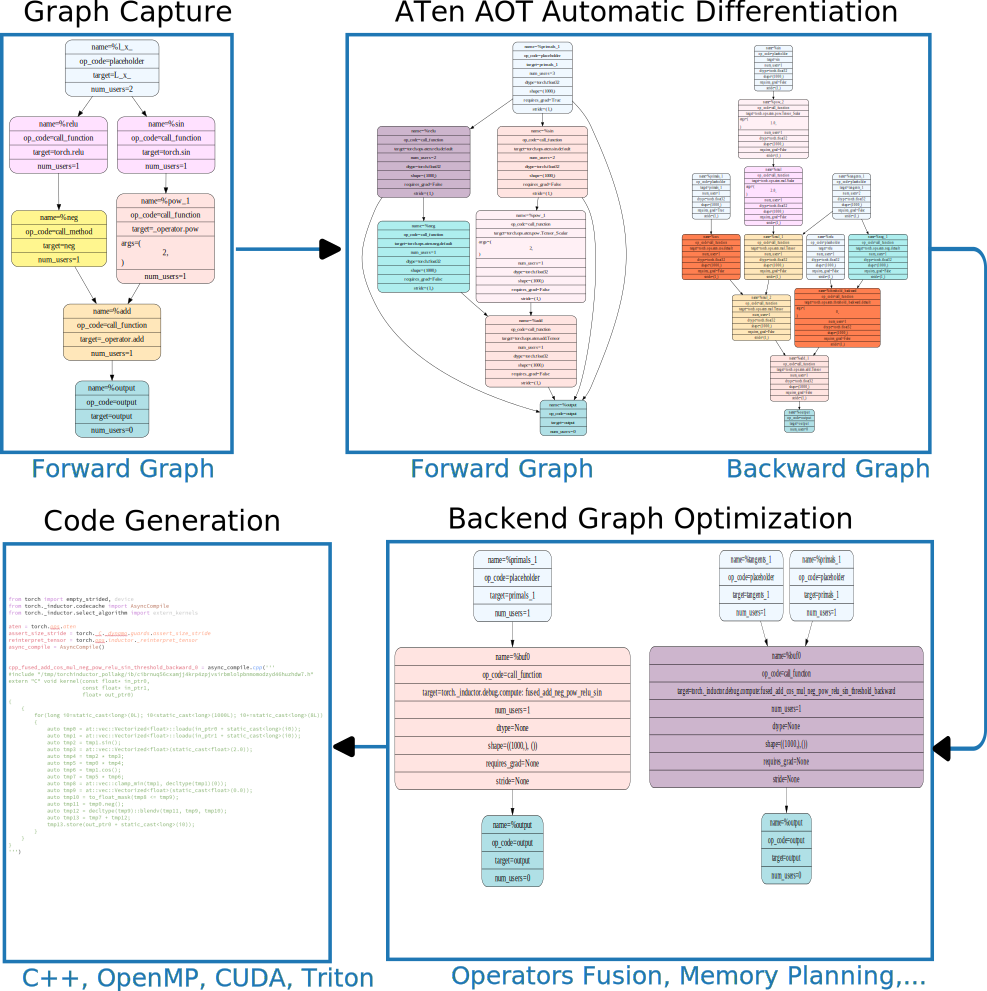
\includegraphics[width=1.0\textwidth]{pytorch_submodule/src/the_framework/graph_acquisition/figures/compile.pdf}
    \end{figure}
\end{sectionbox}
\begin{methodbox}{List Backends}
    \begin{plaincodebox}{python}
    import torch._dynamo as dynamo
    dynamo.list_backends(exclude_tags=('debug', 'experimental'))
    # 'cudagraphs', 'inductor', 'onnxrt', 'openxla', 'openxla_eval', 'tvm'
    \end{plaincodebox}
\end{methodbox}
\begin{notebox}[Backends no longer supported]\nospacing
        \begin{itemizenosep}
            \item nvFuser
        \end{itemizenosep}
\end{notebox}
%%% Local Variables:
%%% mode: latex
%%% TeX-command-extra-options: "-shell-escape"
%%% TeX-master: "../../../../../formulary"
%%% End:
